\question (南开大学,2004年)设n、m为一棵二叉树上的两个结点,在中序遍历时,n在m前的条件是(
)
\par\twoch{n在m的右方}{n是m的祖先}{\textcolor{red}{n在m的左方}}{n是m的子孙}
\begin{solution}中序遍历是左中右的顺序,因此n在m前的条件是n在m的左方。
\end{solution}
\question (南开大学,2005年)对二叉树的结点从1开始进行连续编号,要求每个结点的编号大于其左右孩子的编号,同一结点的左右孩子中,其左孩子的编号小于其右孩子的编号,则可以采用(
)次序的遍历实现编号
\par\twoch{先序}{中序}{\textcolor{red}{后序}}{从根开始按层次遍历}
\begin{solution}``要求每个结点的编号大于其左右孩子的编号'',即先子女后父母,即后序遍历的思想。
\end{solution}
\question (南京理工大学,1999年)设有一表示算术表达式的二叉树,它所表示的算术表达式是(
~)

~
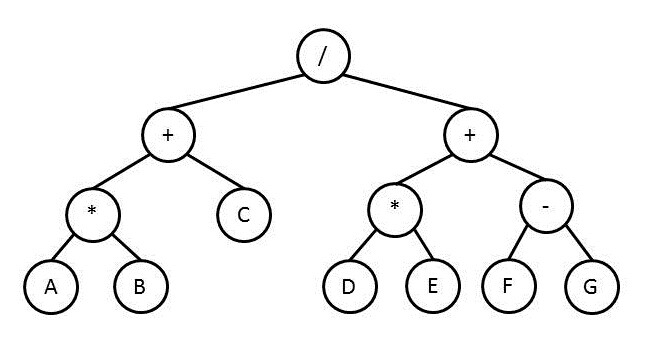
\includegraphics[width=3.12500in,height=1.64583in]{computerassets/529ae776b55a6057f6656794e91069ed.jpeg}
\par\fourch{A*B+C/(D*E)+(F-G)}{(A*B+C)/(D*E)+(F-G)}{\textcolor{red}{(A*B+C)/(D*E+(F-G))}}{A*B+C/D*E+F-G}
\begin{solution}对二叉树进行先序遍历,得到表达式((A*B)+C)/((D*E)+(F-G)),去掉多余的括号后,得到
(A*B+C)/(D*E+(F-G))。
\end{solution}
\question (北京交通大学,2001年)在二叉树结点的先序序列、中序序列和后序序列中,所有叶子结点的先后顺序(
)
\par\twoch{都不相同}{\textcolor{red}{完全相同}}{先序和中序相同,而后序不同}{中序和后序相同,而与先序不同}
\begin{solution}理论上,二叉树有六种遍历方式:NLR、LNR、LRN、NRL、RNL、RLN。
由于前三种次序与后三种次序对称,故只讨论先左后右的前三种次序。因此都是从左子树到右子树进行遍历的,因此所有叶子结点的先后顺序都完全相同。
注:本题也可用排除法。只要随便选一个二叉树写出其三种序列,即可将A,C和D排除。
\end{solution}
\question (北京航空航天大学,1999年)若二叉树采用二叉链表存储结构,要交换其所有分支结点左、右子树的位置,利用(
)遍历方法最合适
\par\twoch{前序}{中序}{\textcolor{red}{后序}}{按层次}
\begin{solution}要实现交换所有分支结点左、右子树的位置,可以递归地进行如下操作:先递归交换左子树中的所有分支结点;再递归交换右子树中的所有分支结点;最后对根结点交换其子树的位置。这对应了先遍历左子树,再遍历右子树,最后访问根结点的后序遍历方式,因此本题选C。
\end{solution}
\question (北京航空航天大学,2002年)已知某完全二叉树采用顺序存储结构,结点数据信息的存放顺序依次为ABCDEFGH,该完全二叉树的后序遍历序列为(
)
\par\twoch{\textcolor{red}{HDEBFGCA}}{HEDBFGCA}{HDEBAFGC}{HDEFGBCA}
\begin{solution}画出该完全二叉树的示意图(下图)后,易得其后序遍历序列为HDEBFGCA,故本题选A。
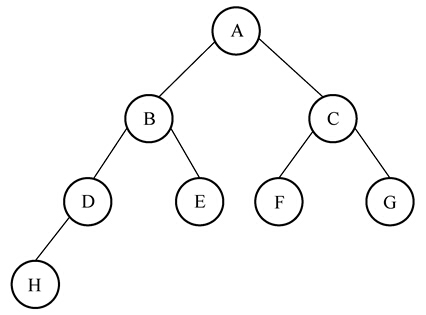
\includegraphics[width=2.08333in,height=2.08333in]{computerassets/82999f59b924ff27710fe8094367a64b.jpeg}
\end{solution}
\question (北京交通大学,2005年)某二叉树的先序序列和后序序列正好相反,则该二叉树一定是(
)
\par\twoch{空或只有一个结点}{\textcolor{red}{高度等于其结点数}}{任一结点无左孩子}{任一结点无右孩子}
\begin{solution}方法一:举特例,先序为123,后序为321,可以得出是棵``独生子女''树(即每个结点最多只有一个孩子的二叉树),本题选B。
方法二:如果A、C、D任意选一个,则B也得选,因为只要A、C、D中任一个成立,B也就成立。因此若本题为单选题,可直接选B。
方法三:高度等于其结点数,即每层只有一个结点,这样NLR就变为先父母后孩子,LRN即先孩子后父母,又因``独生子女''树没有兄弟关系,因此先父母后孩子和先孩子后父母就是逆序关系。
\end{solution}
\question (哈尔滨工程大学,2005年)某n\textgreater{}0个结点的二叉树的先序和后序序列正好相反,则该二叉树一定不是(
)的二叉树
\par\twoch{任一结点无左孩子}{任一结点无右孩子}{深度为n}{\textcolor{red}{存在度为2的结点}}
\begin{solution}D,``独生子女''树满足A、B、C,不满足D。
\end{solution}
\question (中南大学,2003年)某二叉树结点的中序序列为BDAECF,后序序列为DBEFCA,则该二叉树对应的森林包括(
)棵树
\par\twoch{1}{2}{\textcolor{red}{3}}{4}
\begin{solution}先还原二叉树,从后序序列可知根为A,那么左子树的中序就为BD,右子树的中序为ECF,左子树的后序为DB,右子树的后序为EFC;可再得,左子树的根为B,D为右孩子;右子树的根为C,左孩子为E,右孩子为F。画出示意图,如下图所示。
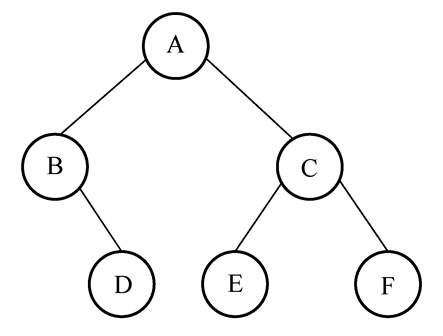
\includegraphics[width=2.08333in,height=2.08333in]{computerassets/bd459a854ebd7c5ece063bf107b6f012.jpeg}
可以直接看根结点有几个兄弟,兄弟数+1(因为还有根结点本身)即为树的个数。
下面给出转换为森林后的示意图:
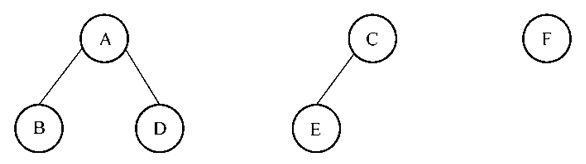
\includegraphics[width=2.08333in,height=2.08333in]{computerassets/02d7f3ef22c9ad637a111d6ad3d5cc3d.jpeg}
综上,本题选C。
\end{solution}
\question (华南理工大学,2006年)一棵二叉树的中序序列为FEABDC,后序序列为FBADCE,则层次序列为(
)
\par\twoch{ABCDEF}{EFCDBA}{FECDAB}{\textcolor{red}{EFCDAB}}
\begin{solution}根据后序序列E在最后,则E为根结点,由中序序列判断F为E的唯一左结点,E的右子树的中序序列为ABDC,后序序列为BADC,则根为C,C的左子树的中序序列为ABD,后序序列为BAD,根为D,左子树的中序序列为AB,后序序列为BA,则根为A,B为右孩子。得到的二叉树结构如下图所示:
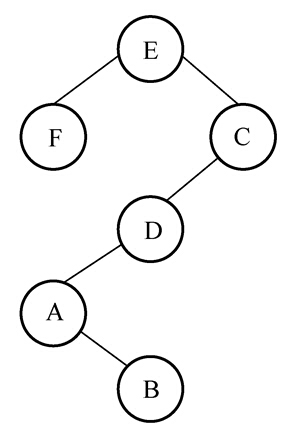
\includegraphics[width=2.08333in,height=2.08333in]{computerassets/b6adf4b2fc3f392b6f1c076f3cde5135.jpeg}
\end{solution}
\question 给定二叉树如下图所示。设N代表二叉树的根,L代表根结点的左子树,R代表根结点的右子树。若遍历后的结点序列为3,1,7,5,6,2,4,则其遍历方式是(
~)。

~
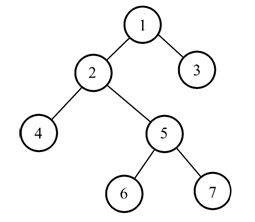
\includegraphics[width=1.04167in,height=0.90625in]{computerassets/449D7634892FD3CB3AEC7CABC2C24708.png}
\par\twoch{LRN}{NRL}{RLN}{\textcolor{red}{RNL}}
\begin{solution}根据遍历结果,很容易看出右子树先被访问,再根结点,最后左子树,相当于左右颠倒的中序遍历,即为RNL。
本题的其他3种遍历序列如下:
(1)LRN(先左子树,再右子树,最后访问根结点):4,6,7,5,2,3,2。
(2)NRL(先访问根结点,再右子树,最后左子树):1,3,2,5,7,6,4。
(3)RLN(先右子树,再左子树,最后访问根结点):3,7,6,5,4,2,1。
【总结】
已知二叉树结构和遍历方式,求遍历序列;已知二叉树结构和遍历序列,推测遍历方式,这都属于二叉树遍历中最基本的题目。
\end{solution}
\question 若一棵二叉树的前序遍历序列为a,e,b,d,c,后序遍历序列为b,c,d,e,a,则根结点的孩子结点(
)
\par\twoch{\textcolor{red}{只有e}}{有e、b}{有e、c}{无法确定}
\begin{solution}根节点一定是a,就有3种可能: ①a有左孩子,无右孩子。
②a无左孩子,有右孩子。 ③a有左孩子,有右孩子。
假设情况一成立,e,b,d,c即为左子树的先序序列,b,c,d,e即为左子树的后序序列,明显e为左子树的根节点,且左右孩子皆有(考虑单个子树的话,先序bdc与后序bcd矛盾)。故该左子树可能如下图所示。
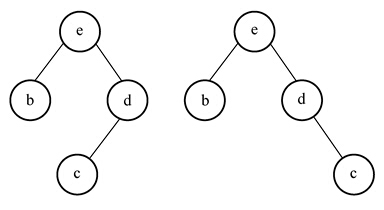
\includegraphics[width=4.00000in,height=2.18750in]{computerassets/8477d425f479b1f532486ea3861e03b0.jpeg}
假设情况二成立,得出e为右子树的根节点,右子树的可能情况也同上。
假设情况三成立,e即为左子树,b、d、c即为右子树的先序序列,b、c、d即为右子树的后序序列,该先序序列与后序序列矛盾。
所以该二叉树只有一个孩子结点e。 【总结】
由二叉树的中序序列和后序序列、中序序列和先序序列、中序序列和层次序列都可以唯一确定一棵二叉树。但不能由先序序列和后序序列唯一确定一棵二叉树。
任意两个先序序列和后序序列,不能唯一确定一棵二叉树,如本题的情况。同时,也可能没有一棵二叉树符合这两种遍历序列。如先序ab,后序ab即无二叉树与之对应。
\end{solution}
\question (哈尔滨工程大学,2005年)某n\textgreater{}0个节点的二叉树的先序序列和后序序列正好相反,则该二叉树一定不是(
)的二叉树
\par\twoch{任一节点无左孩子}{任一节点无右孩子}{深度为n}{\textcolor{red}{存在度为2的节点}}
\begin{solution}ABC均可能成立,但如果存在度为2的节点,则先序与后序序列不可能正好相反
\end{solution}
\question (南开大学,2005年)对二叉树的节点从1开始进行连续编号,要求每个节点的编号大于其左右孩子的编号,同一节点的左右孩子中,其左孩子的编号小于其右孩子的编号,则可以采用(
)次序的遍历实现编号
\par\twoch{先序}{中序}{\textcolor{red}{后序}}{从根开始按层遍历}
\begin{solution}考察几种遍历到额差异,后序遍历时,是按照左右根的顺序遍历,则满足从小到大的顺序,这样就可以对其依次编号即可
\end{solution}
\question (南开大学,2004年)设n,m为一棵二叉树上的两个节点,在中序遍历时,n在m前的条件是(
)
\par\twoch{n在m右方}{n是m的祖先}{\textcolor{red}{n在m的左方}}{n是m的子孙}
\begin{solution}首先可以排除BD,因为中序遍历祖先与子孙的遍历顺序取决于子孙是左子树还是右子树。根据左中右的遍历顺序可知n在m的左方
\end{solution}
\question (北京交通大学,2005年)某二叉树的先序序列和后序序列正好相反,则该二叉树一定是(
)
\par\twoch{空或者只有一个节点}{\textcolor{red}{高度等于其节点数}}{任一节点无左孩子}{任一节点无右孩子}
\begin{solution}考察二叉树的先序遍历序列和后序遍历序列,先序遍历是根左右,后序遍历是左右根,很明显只有每个节点(叶子节点除外)只有一个孩子的时候,先序序列正好和后序序列相反
\end{solution}
\question (山东大学,2005年)任何一棵二叉树的叶子节点在先序中序和后序中的相对次序(
)
\par\twoch{\textcolor{red}{不发生改变}}{发生改变}{不能确定}{以上都不对}
\begin{solution}无论是先序中序还是后序,都是按照先左后右的顺序进行访问,所以叶子节点遍历过程的相对顺序是固定的
\end{solution}
\question (哈尔滨工程大学,2004年)二叉树用二叉链表表示,若要将其所有节点的左右子树交换位置,则采用下列(
)遍历的方法比较合适
\par\twoch{先序}{中序}{\textcolor{red}{后序}}{层序}
\begin{solution}首先按层序遍历是最不可取的方法,因为树是用二叉链表表示的,按层交换的查找会非常麻烦;中序遍历遵循左、中、右的原则,但是在左子树交换结束之后,遍历至根节点会交换左右子树的位置,需要交换的右子树便无法被遍历到;先序和后序都可以完成左右子树交换的工作,但是先序的话并不是正真意义上的``先序'',因为把根节点的左右子树交换之后,此时访问的左子树是原来树的右子树。综上只有后序最贴切
\end{solution}
\question (哈尔滨工程大学,2004年)对于二叉树的两个节点x和y,应该选择(
)两个序列来判断x是否为y的祖先
\par\twoch{先序和后序}{先序和中序}{中序和后序}{\textcolor{red}{任意两个序列}}
\begin{solution}虽然由先序和后序无法的出二叉树的结构,但是可以判断祖先,(在先序序列中和后序序列中看x和y的相对位置是不是正好相反),其他两个可以直接得出树结构则可以判断祖先
\end{solution}
\question (江苏大学,2004年)对二叉排序树进行(
)遍历,可以得到该二叉树所有节点构成的排序序列
\par\twoch{前序}{\textcolor{red}{中序}}{后序}{层次}
\begin{solution}考察二叉排序的树的特征以及二叉树的中序遍历,只有中序遍历才是按照节点的关键字的大小递增排序
\end{solution}
\question (重庆大学,2005年)已知某二叉树的先序序列为ABDCE,它可能的中序序列为(
)
\par\twoch{\textcolor{red}{BDAEC}}{BCAED}{CBADE}{BEACD}
\begin{solution}二叉树的先序序列可以分为连续的3部分:第一个是根节点,后面分别是左子树部分和右子树部分,中序遍历也可以分为3部分:左子树部分、根节点、右子树部分。题目给得出的先序序列为ABDCE,可知A为根节点,A给出的中序序列表示BD是左子树部分,EC是右子树部分,和先序序列不矛盾,是可能的中序序列。B给出的序列表示BC是左子树,DE是右子树,这两个部分在先序序列ABDCE中不连续,说明不是可能的中序序列。同理,C和D也不是
\end{solution}
\question (重庆大学,2004年)一棵二叉树节点的( )可唯一确定一棵二叉树
\par\twoch{\textcolor{red}{前序序列和中序序列}}{前序序列和后续序列}{中序序列}{后序序列}
\begin{solution}能唯一确定原二叉树的遍历方式组合是:前序+中序,或者是后序+中序,而前序+后序不能确定唯一的二叉树
\end{solution}
\question (重庆大学,2004年)已知某二叉树的后序遍历序列是dabec,中序遍历序列是debac,它的前序遍历序列是(
)
\par\twoch{acbed}{decab}{deabc}{\textcolor{red}{cedba}}
\begin{solution}根据后序遍历序列和中序遍历序列构建二叉树,然后得出它的前序遍历序列
\end{solution}
